\chapter{Our approach}
In authorship attribution problems, there is a set of candidate authors and a set of
text samples in the training set covering some of the works of the authors. In the
test dataset, there are sample of texts and each of them needs to be attributed to
a candidate author.
In the next sections, we are going to describe the experiment we carried out taking care of the chronological path of the events.
Our main focus has always been on closed set authorship attribution, training with instance-based approach (i.e. extracting features by not considering the other available text samples in the training).
The three milestones can be summarized as follows:
\begin{enumerate}
	\item Dataset selection and preparation
	\item Classifier method's selection
	\item Features extraction
\end{enumerate}

\section{Dataset preparation}
In section 4.6 we have already shown the datasets we selected. In particular, in this section we are going to show the procedures done to prepare the datasets for the next steps. For the single topic authorship attribution task we decided to select the RCV1 dataset, the dataset of 45 Victorian era book authors from the GDELT project and the dataset of amazon food reviews collected in the first decade of the 2000s. Regarding the cross domain authorship attribution task, we selected the dataset extracted from The Guardian newspaper.

\subsection{Reuters Corpus (RCV1)}
It consists of a collection of newswire stories written in English that cover four main topics: corporate/industrial (CCAT), economics (ECAT), government/social (GCAT) and markets (MCAT).
We sent a request to obtain the dataset on this webpage \url{https://trec.nist.gov/data/reuters/reuters.html}.
After few days, we gathered the RCV1 Corpus as it contains 810,000 Reuters, English Language News stories (about 2.5 GB).
First of all we had to convert the dataset, that contained folders of xml files, into a big csv with author's labels and document text.
\autoref{lst:RCV1Extraction} shows the process of documents and authors extraction, using `xml` python library. We decided to take into account this properties of the document: \textit{text, title, headline, byline, dateline, lang, corpus\_path, corpus\_subdirectory, corpus\_filename}.


\begin{lstlisting}[frame=none,caption={Extract and Parse RCV1 XML document into csv},captionpos=b,label=lst:RCV1Extraction]
\end{lstlisting}
\begin{python}	
	import os
	import xml.etree.ElementTree as ET

	for f in files:
		try:
			data_path = os.sep.join([dir_path, f])
			raw_data = open(data_path).read()
			try:
				xml_parse = ET.fromstring(raw_data)
			except:
				print(D,"/",f,"failed to parse XML.")
				continue
		
			def get_text(tag): 
				stuff = xml_parse.find(tag)
				if stuff: 
					return stuff.text
				else: 
					return None
	
		text = "\n\n".join([str(p.text) for p in xml_parse.findall(".//p")])
		title = get_text("title")
		headline = get_text("headline")
		byline = get_text("byline")
		dateline = get_text("dateline")
		
		#this bit got funky in the XML parse
		lang_key = [k for k in xml_parse.attrib if "lang" in k][0]
		lang = xml_parse.attrib[lang_key]
	
		code_classes = [c.attrib["class"] 
		for c in xml_parse.findall(".//codes")]
		codes = {cc: [c.attrib["code"] for c in 
			xml_parse.findall(".//codes[@class='%s']/code"%cc)]
			for cc in code_classes}
		dcs = {d.attrib["element"]: d.attrib["value"] 
			for d in xml_parse.findall(".//dc")}
		
		#assemble output
		output = {"text": text,
			"title": title,
			"headline": headline,
			"byline": byline,
			"dateline": dateline,
			"lang": lang,
			"corpus_path": corpus_path,
			"corpus_subdirectory": D,
			"corpus_filename": f,
		}
		
		# merge and flatten the other big hashmaps
		output.update(codes.items())
		output.update(dcs.items())
		
		result.append(output)
	except Exception as e:
		print(e)
\end{python}

The dataset was then filtered only with the documents with a \textit{"byline"} property defined. We end up with 109'433 documents written by 2400 distinct authors. At this point, we labeled this portion of the RCV1 original dataset as the \textit{"Full RCV1 dataset"}.
In order to test and compare our approach, reproducing the testing scenario
described in the previous research \cite{stamatatos2009survey}, the 10 most prolific authors were chosen from the CCAT category, and then, 50 examples per author for training and 50 examples for testing were selected randomly with no overlapping between training and testing sets. We will reference to this portion of the RCV1 dataset as the \textit{"RCV1\_10"}.
In previous work \cite{houvardas2006n}, the authors proposed another adaptation of the RCV1 corpus for the authorship attribution task. They choose the 50 most prolific authors from the Reuters Corpus, keeping 50 examples per author for training and 50 examples per author for testing with no
overlapping between them. We will refer to this corpus as the \textit{RCV1\_50}.\\
The RCV1\_10 and RCV1\_50 datasets are both balanced over different authors and have their genre fixed to news.
The majority of our work has been conducted on the RCV1\_50, although to compare results with previous works we will show also the same techniques applied to the RCV1\_10 corpus.
\autoref{tab:tableRCV1kpi} shows the main metrics to describe these different portions of the original dataset.

\begin{table}[h!]
	\begin{center}  
		\caption[RCV1 Corpus]{Main metrics to describe different portion of the dataset} 
		\label{tab:tableRCV1kpi}
		%\resizebox{\linewidth}{!}{  %
		\begin{tabular}{|c | c | c | c | c |}
			\hline 
			Name & N\# documents & N\# authors & Avg docs length & Avg n\# docs/author \\
			\hline
			Full RCV1 dataset & 109433 & 2400 & 3061.95 & 45.60 \\ \hline
			RCV1\_10 & 1000 & 10 & 3093.82 & 100  \\ \hline
			RCV1\_50 & 5000 & 50 & 3251.16 & 100  \\ \hline
			%\bottomrule 
		\end{tabular} 
		%}
	\end{center}
\end{table}

\subsection{GDELT}
The GDELT Project is one of the largest publicly available digitized book database
which has more than 3.5 million books published from 1800-2015.
To decrease the bias and create a reliable dataset the following criteria have been
chosen to filter out authors: English language writing authors, authors that have
enough books available (at least 5), 19th century authors. With these criteria 50
authors have been selected and their books were queried through Big Query Gdelt
database. The next task has been cleaning the dataset due to OCR reading problems
in the original raw form. To achieve that, firstly all books have been scanned through
to get the overall number of unique words and each words frequencies. While scanning
the texts, the first 500 words and the last 500 words have been removed to take out
specific features such as the name of the author, the name of the book and other word
specific features that could make the classification task easier. After this step, we have
chosen top 10, 000 words that occurred in the whole 50 authors text data corpus. The
words that are not in top 10, 000 words were removed while keeping the rest of the
sentence structure intact 2 . Afterwards, the words are represented with numbers from
1 to 10, 000 reverse ordered according to their frequencies. The entire book is split
into text fragments with 1000 words each. We separately maintained author and
book identification number for each one of them in different arrays. Text segments
with less than 1000 words were filled with zeros to keep them in the dataset as well.
1000 words make approximately 2 pages of writing, which is long enough to extract a variety of features from the document. The reason why we have represented top
10, 000 words with numbers is to keep the anonymity of texts and allow researchers
to run feature extraction techniques faster. Dealing with large amounts of text data
can be more challenging than numerical data for some feature extraction techniques.
When gathering the dataset, we decided to discard 5 authors for which their writings were not enough consistent for the authorship attribution task.
We ended up with a full dataset with 53'678 documents instances, each one containing 1000 words.
In order to make training's methods reliable across dataset, we decided to select 100 documents of each authors, with a 50/50 split (i.e. 50 documents in the training set, 50 documents in the testing set, no overlapping among them). In the following sections, we will refer to this as the \textit{"GDELT\_45"}.
\autoref{tab:tableGDELTkpi} shows the metrics that describe best this dataset.

\begin{table}[h!]
	\begin{center}  
		\caption[GDELT Corpus]{Main metrics to describe different portion of the GDELT dataset} 
		\label{tab:tableGDELTkpi}
		%\resizebox{\linewidth}{!}{  %
		\begin{tabular}{|c | c | c | c | c |}
			\hline 
			Name & N\# documents & N\# authors & Avg docs length & Avg n\# docs/author \\
			\hline
			Full GDELT dataset & 53678 & 45 & 4950.61 & 1192.84 \\ \hline
			GDELT\_45 & 4500 & 45 & 4911.91 & 100  \\ \hline
			%\bottomrule 
		\end{tabular} 
		%}
	\end{center}
\end{table}

\subsection{Amazon Food Reviews (AFR)}
This dataset consists of reviews of fine foods from amazon. The data span a period of more than 10 years, including all ~500,000 reviews up to October 2012. Reviews include product and user information, ratings, and a plain text review. It also includes reviews from all other Amazon categories.
We decided to consider this dataset for our experiment, because we were missing a more "everyday" example of dataset to work with. As \autoref{tab:tableAFRkpi} shows, among the main metrics, that the average documents length is dramatically lower than the other two dataset presented previously, providing a good challenge for us to show consistency of our method across all these different scenarios.
Moreover, in order to make training's methods reliable across dataset, we decided to select 100 reviews of each customers, with a 50/50 split (i.e. 50 reviews in the training set, 50 reviews in the testing set, no overlapping among them). In the following sections, we will refer to this as the \textit{"AFR\_50"}.

\begin{table}[h!]
	\begin{center}  
		\caption[AFR Corpus]{Main metrics to describe different portion of the AFR dataset} 
		\label{tab:tableAFRkpi}
		%\resizebox{\linewidth}{!}{  %
		\begin{tabular}{|c | c | c | c | c |}
			\hline 
			Name & N\# documents & N\# authors & Avg docs length & Avg n\# docs/author \\
			\hline
			Full AFR dataset & 568454 & 256059 & 380.70 & 2.2 \\ \hline
			AFR\_50 & 5000 & 50 & 990.45 & 100  \\ \hline
			%\bottomrule 
		\end{tabular} 
		%}
	\end{center}
\end{table}

\subsection{The Guardian newspaper}
Although the majority of our time and effort was focused on the first 3 single domain closed set authorship attribution task, we wanted to test our approach with a cross domain dataset.
\textit{The Guardian corpus} is composed of texts published in The Guardian daily newspaper. The majority of the corpus comprises opinion articles
(comments). The newspaper describes the opinion articles using a set of tags indicating its subject. There are eight top-level tags (World, U.S., U.K., Belief, Culture, Life\&Style, Politics, Society), each one of them having multiple subtags.
In order to test and compare our approach, we reproduce the testing scenario
described in the previous research \cite{stamatatos2013robustness} using the Guardian corpus. The experimental
scenario is as follows: 
\begin{enumerate}
	\item Select at most ten samples per author in each topic category
	(in \autoref{fig:tgc_dataset} the distribution of the samples per author for the Politics category after considering
	the restriction of ten samples per author is shown)
	\item Use the samples in the Politics category as training set and train the classifier
	\item Finally, test the classifier using
	another topic category different from Politics (four possible pairings)
\end{enumerate}

\begin{figure}[ht]
	\centering
	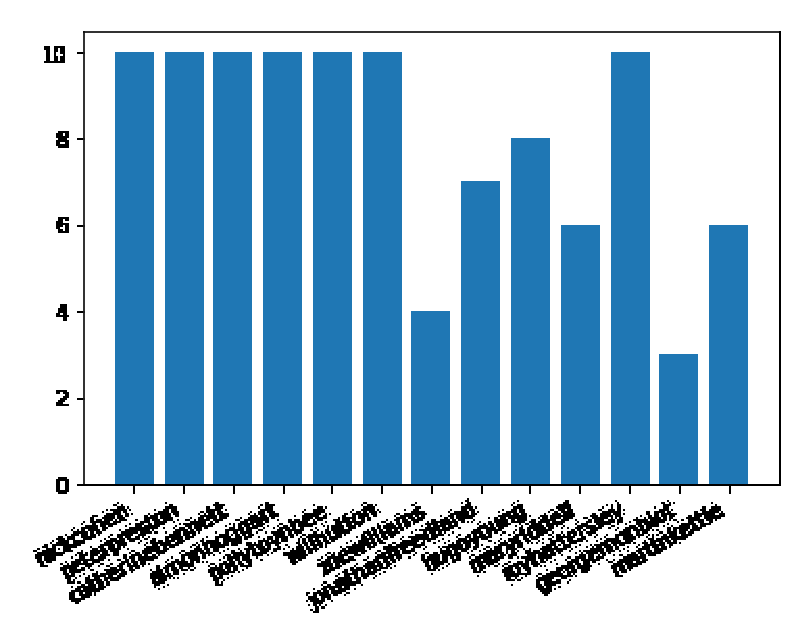
\includegraphics[width=.6\textwidth, height=.6\textheight, keepaspectratio]{theguardian_dataset}
	\caption[The Guardian Politics samples distribution]{The Guardian samples distribution for the Politics topic}
	\label{fig:tgc_dataset}
\end{figure}

\section{Method's selection}
At this point, we had to face the problem of deciding the classifier method that would solve best our authorship attribution task.
Although in previous studies over the past decades on authorship attribution SVM has been shown to be very convincing (\cite{diederich2003authorship}, \cite{koppel2005determining}, \cite{zheng2006framework}), we initially wanted to construct an experimental approach that would lead us to exclude the other classifiers for our task.
\subsection{Naive Approach}
Our very first naive approach was to compare on different portions of the dataset (increasing number of authors) different classification methods to see which one performed best.
Initially, we considered the author attribution study for groups of authors consisting of 6 or 10 authors. In truth, as many previous studies show, an author attribution model must perform well especially in situations where the group of authors is composed of several dozen candidates.
The classifiers initially chosen were:
\begin{itemize}
	\item Naive Bayes
	\item Multinomial Naive Bayes
	\item Logistic Regression
	\item XGBoost
	\item XGBoost with Neural Networks
	\item Random Forest
\end{itemize}
For text representation, we chose to use TFIDF and Bag Of Words, comparing the results depending on the dataset, the number of authors, and the method used.
In \autoref{fig:RCV1_methods_accuracy} we can see the accuracy score of the testing set of the various classifiers tested on the groups of authors increasing from right to left on the RCV1 dataset.
As on the groups of "small" authors, i.e. composed of 6 authors and 10 authors, almost all the classifiers exceed the threshold of 95\% accuracy that validates the approach even in non-research contexts. The classifier that seems to perform best among the various groups of authors increasing in number is RandomForest. On the other hand, it has been shown that decision tree type classifiers struggle to maintain high performance when the number of features used increases.

\begin{figure}[ht]
	\centering
	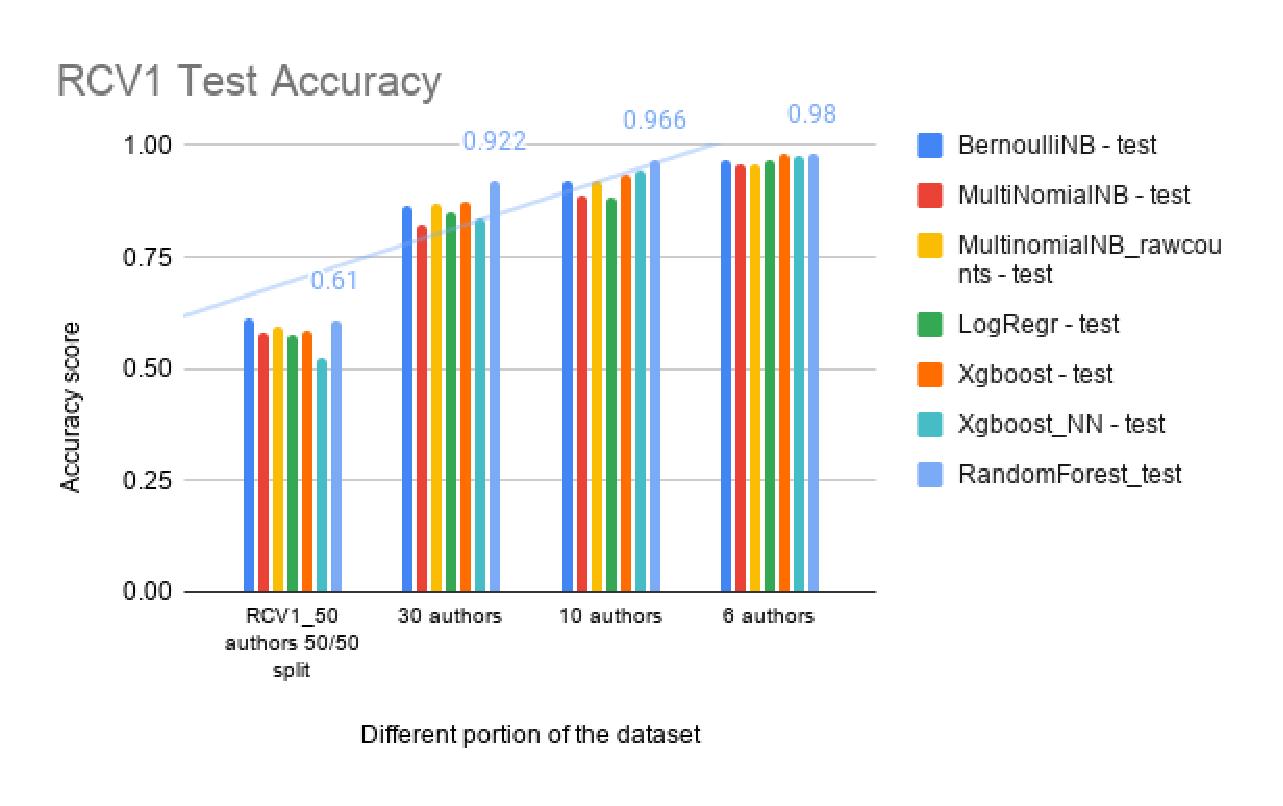
\includegraphics[width=.8\textwidth, height=.8\textheight, keepaspectratio]{RCV1_Test_Accuracy}
	\caption[Methods performance on RCV1]{Accuracy scores for different groups of authors on RCV1 dataset}
	\label{fig:RCV1_methods_accuracy}
\end{figure}

In fact in \autoref{fig:GDELT_methods_accuracy} and \ref{fig:AFR_methods_accuracy} we can see that in all 3 single topic datasets the various methods proposed have a decrease in performance when the number of authors increases reaching 50 authors (or 45 in the case of the GDELT dataset).
This is probably due to the fact that by keeping the number of documents per author fixed at 50 in the training test (and in the testing set), the number of features to represent grows disproportionately as the number of authors increases. Therefore, we need to select a classification method that remains stable as the number of features we want to represent increases, and therefore remains valid for 6, 10, 30, 50 authors (and more).

\begin{figure}[ht]
	\centering
	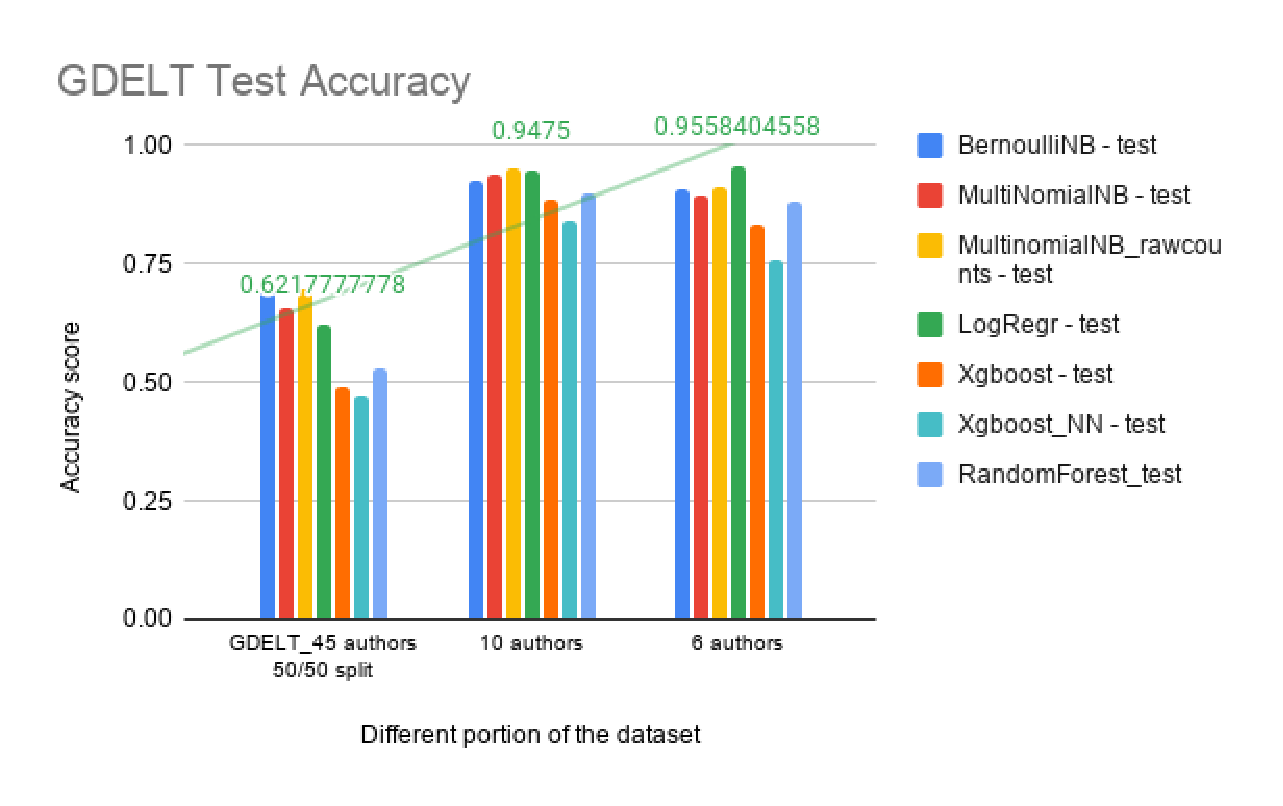
\includegraphics[width=.8\textwidth, height=.8\textheight, keepaspectratio]{GDELT_Test_Accuracy}
	\caption[Methods performance on GDELT]{Accuracy scores for different groups of authors on GDELT dataset}
	\label{fig:GDELT_methods_accuracy}
\end{figure}

\begin{figure}[ht]
	\centering
	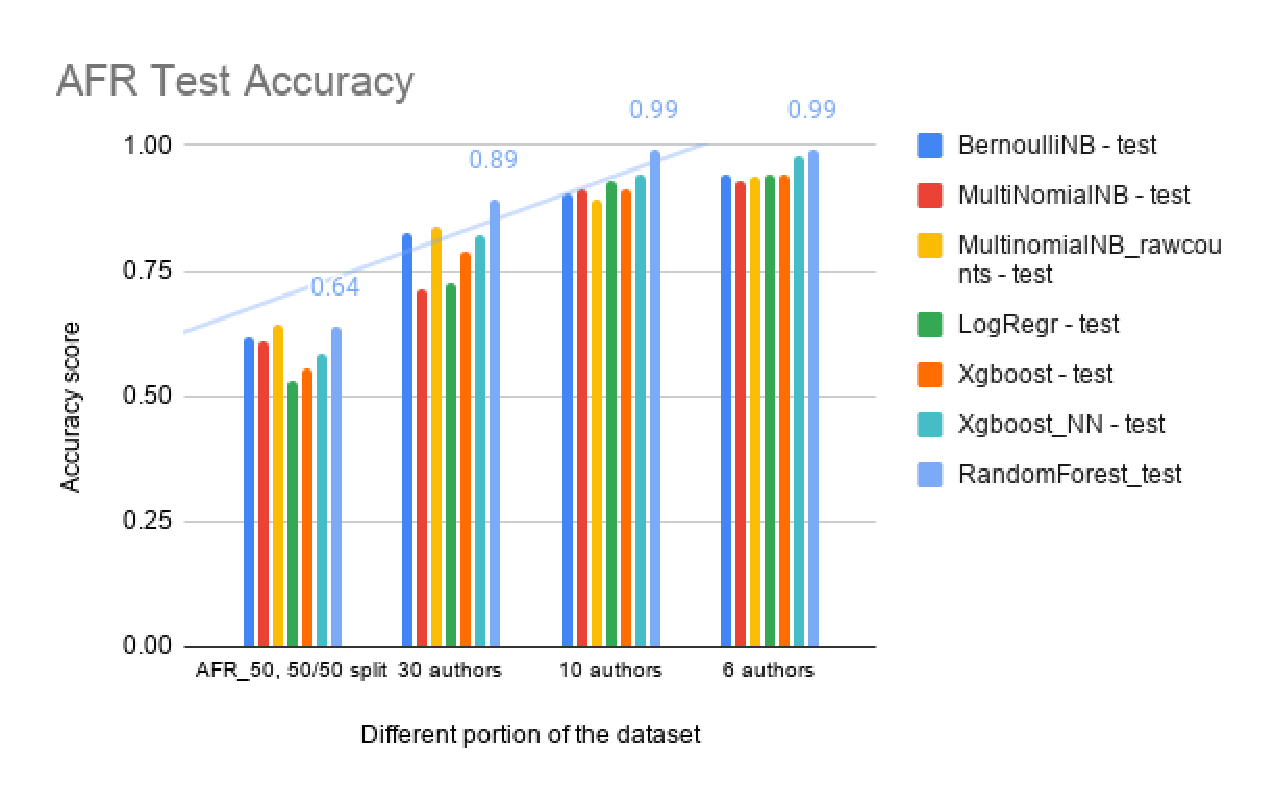
\includegraphics[width=.8\textwidth, height=.8\textheight, keepaspectratio]{AFR_Test_Accuracy}
	\caption[Methods performance on AFR]{Accuracy scores for different groups of authors on AFR dataset}
	\label{fig:AFR_methods_accuracy}
\end{figure}

\subsection{TeaPot}

\section{Features extraction}
\subsection{TFIDF \& BOW}
\subsection{GridSearchCV}
\subsection{Doc2Vec}

